\documentclass{beamer}
 
\usepackage[utf8]{inputenc}
\usetheme{Warsaw}
\usecolortheme{beaver}
 
%Information to be included in the title page:
\title{Classification with Restricted Boltzmann Machines}
\subtitle{Projects in Machine Learning and AI}
\author{Fritjof Wolf \\ Katarzyna Tarnowska}
\institute{Technische Universitat Berlin}
\date{2015}
\logo{
\includegraphics[height=1.5cm]{images/TUBerlin.png}}



\begin{document}

  \AtBeginSection[]
  {
    \begin{frame}
      \frametitle{Table of Contents}
      \tableofcontents[currentsection]
    \end{frame}
  }
  
  \AtBeginSubsection[]
  {
    \begin{frame}
      \frametitle{Table of Contents}
      \tableofcontents[currentsubsection]
    \end{frame}
  }
  \begin{frame}[plain]
    \titlepage
  \end{frame}
  \section{Theory}
  %sample subsections
  \subsection{Boltzmann Machines} 
  \begin{frame}
    \frametitle{Sample frame title}
    \framesubtitle{A bit more information about this}
    This is a text in first frame. This is a text in first frame. This is a text in first frame.
  \end{frame}
  \subsection{Restricted Boltzmann Machines}
  \begin{frame}
  \frametitle{Some useful math equations}
  %Energy function
  \begin{align}
      \mathbf{E(v,h) = \sum_{i=1}^{V} \frac{(v_i - b_i^v)^2}{2\sigma_i^2} - \sum_{j=1}^{H} b_j^h h_j - \sum_{i=1}^{V} \sum_    {j=1}^{H} \frac{v_i}{\sigma_i} h_j w_ij}
  \end{align}

  %Probability of (v,h)
  \begin{align}
      \mathbf{p(v,h) = \frac{e^{-E(v,h)}}{\sum_x \sum_k e^{-E(x,k)}}}
  \end{align}
  \end{frame}
  \subsection{Contrastive Divergence} 
  \section{Implementation}
  \begin{frame}[plain]
  \frametitle{Implementation}
  \begin{columns}
        \begin{column}{0.3\textwidth}
            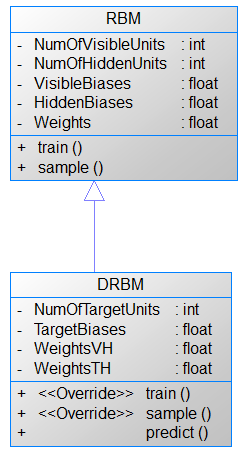
\includegraphics[width=3cm]{images/classDiagram.png}
        \end{column}
        \begin{column}{0.7\textwidth}
			\centering
			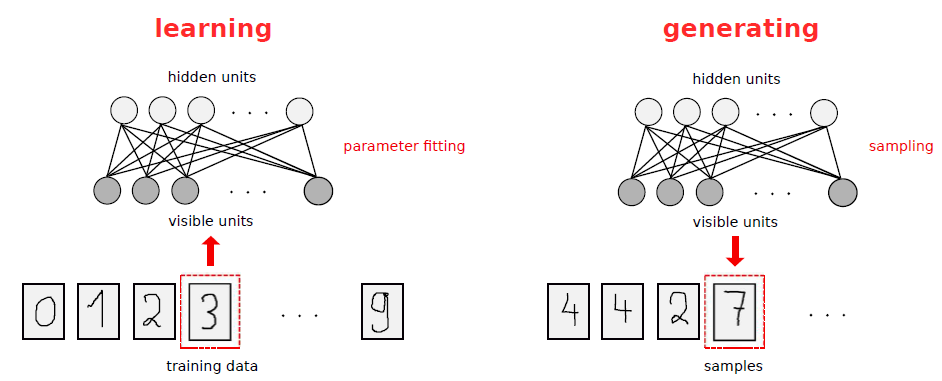
\includegraphics[width = 7cm]{images/generativeRBM.png}
			\captionof{\TINY GRBM}
			{\TINY Source: A.Fischer, Ch.Igel: Training Restricted Boltzmann Machines: An Introduction}
			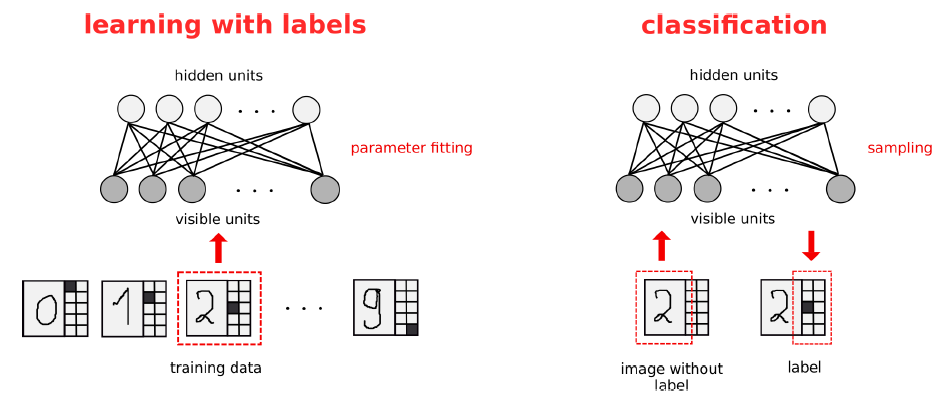
\includegraphics[width = 7cm]{images/DRBM.png}
			\captionof{\TINY DRBM}
			{\TINY Source: A.Fischer, Ch.Igel: Training Restricted Boltzmann Machines: An Introduction}
        \end{column}
    \end{columns}
  \end{frame}
  \section{Results}
  \begin{frame}[allowframebreaks]
  \frametitle<presentation>{Further Reading}    
  \begin{thebibliography}{10}    
  \beamertemplatebookbibitems
  \bibitem{Autor1990}
    A.~Autor.
    \newblock {\em Introduction to Giving Presentations}.
    \newblock Klein-Verlag, 1990.
  \beamertemplatearticlebibitems
  \bibitem{Jemand2000}
    S.~Jemand.
    \newblock On this and that.
    \newblock {\em Journal of This and That}, 2(1):50--100, 2000.
  \end{thebibliography}
  \end{frame}
\end{document}
